\subsection{Cinemática directa}
\subsubsection{Método geométrico}
La proyección radial y la altura relativa del efector son
\begin{equation}
\rho=l_2c_2+l_3c_{23},\qquad z_r=l_2s_2+l_3s_{23}.
\end{equation}
Por proyección sobre la base se obtiene
\begin{equation}
P_{03}=\begin{bmatrix}p_x\\p_y\\p_z\end{bmatrix}=
\begin{bmatrix}c_1\rho\\s_1\rho\\l_1+z_r\end{bmatrix}.
\end{equation}
$\rho$ es una coordenada radial con signo; $\sqrt{p_x^2+p_y^2}=|\rho|$.

\subsubsection{Transformaciones homogéneas y DH}
La construcción por rotaciones y traslaciones de la semana 4 se adapta al RRR mediante \parencite{course4}
\begin{align}
M_{01}&=R_z(\theta_1)T_z(l_1)R_x(\pi/2),\\
M_{12}&=R_z(\theta_2)T_x(l_2),\qquad
M_{23}=R_z(\theta_3)T_x(l_3),\\
M_{03}&=M_{01}M_{12}M_{23}.
\end{align}
La convención DH es $R_z(\theta)T_z(d)T_x(a)R_x(\alpha)$, con los parámetros:
\begin{center}\begin{tabular}{ccccc}\toprule
Trama & $\theta$ & $d$ & $a$ & $\alpha$\\\midrule
$0\to1$ & $\theta_1$ & $l_1$ & 0 & $\pi/2$\\
$1\to2$ & $\theta_2$ & 0 & $l_2$ & 0\\
$2\to3$ & $\theta_3$ & 0 & $l_3$ & 0\\\bottomrule
\end{tabular}\end{center}
El producto da
\begin{equation}
M_{03}=\begin{bmatrix}
c_1c_{23}&-c_1s_{23}&s_1&c_1\rho\\
s_1c_{23}&-s_1s_{23}&-c_1&s_1\rho\\
s_{23}&c_{23}&0&l_1+z_r\\
0&0&0&1
\end{bmatrix}.
\end{equation}
La columna de posición coincide con el método geométrico. El código compara también una implementación de transformaciones elementales con la función DH, y comprueba $R^TR=I$ y $\det R=1$. Se reconstruyen las matrices en lugar de propagar las inconsistencias tipográficas del artículo.

\subsubsection{Espacio de trabajo}
Como en la semana 7, se recorren combinaciones de ángulos y se calcula $P_{03}$ en cada una. Se emplean 21 valores por articulación, con rangos ilustrativos $[-140,140]^\circ$, $[-120,120]^\circ$ y $[-110,110]^\circ$: 9261 posiciones. Estos rangos son un escenario de estudio, no límites mecánicos documentados del VSL.
\begin{figure}[htbp]\centering
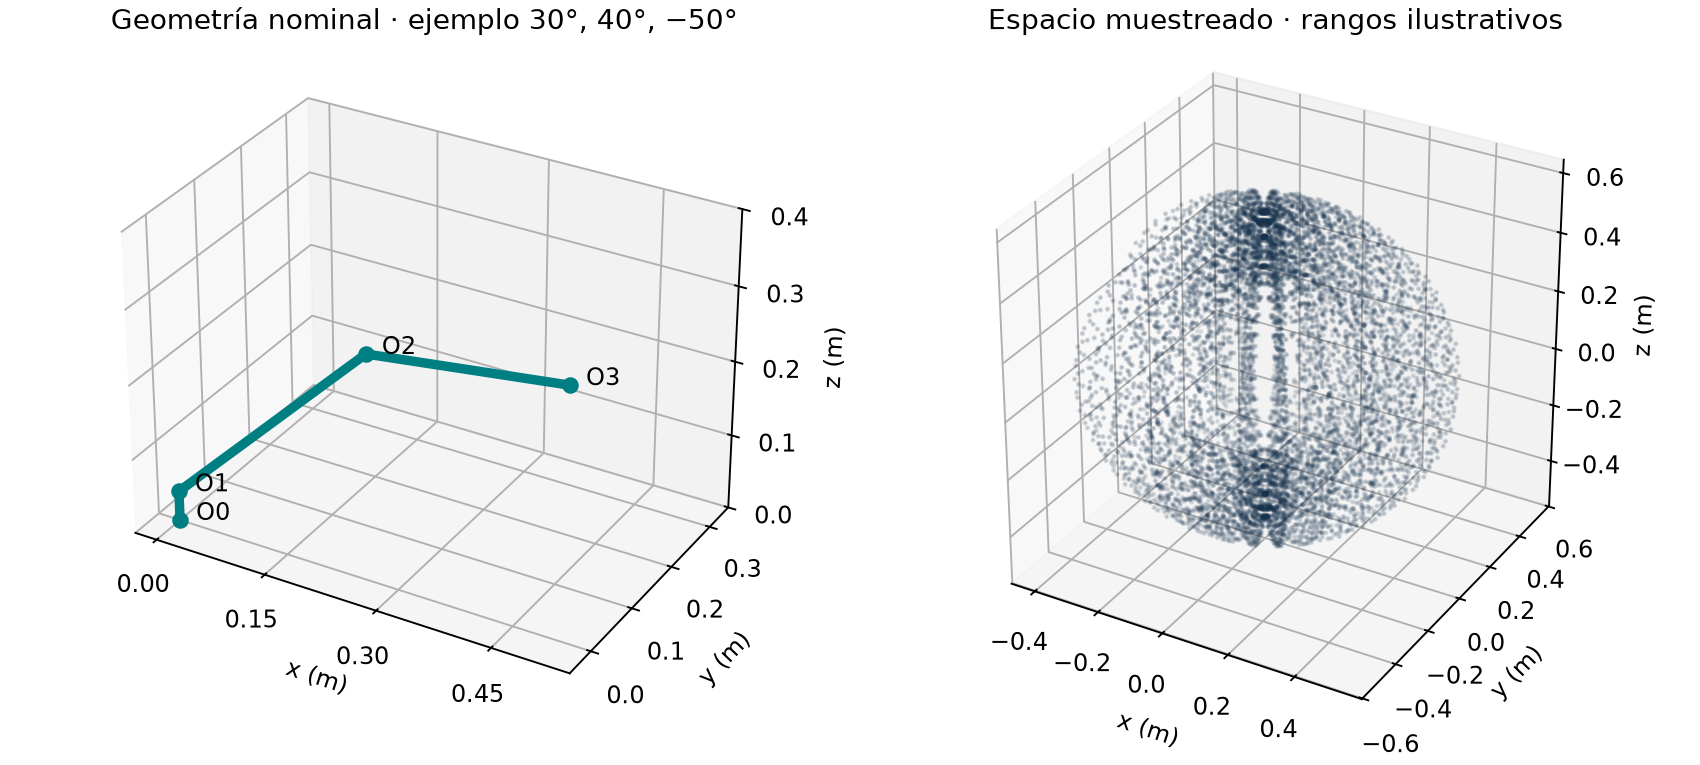
\includegraphics[width=\linewidth]{../simulations/course/results/run-001/workspace.png}
\caption{Geometría y espacio muestreado del modelo nominal. Elaboración propia.}
\end{figure}
